% ================================================================
% chapters/chapter3.tex --- RECONSTRUCTION (v2, remarques encadrant)
% ----------------------------------------------------------------
% APPLIQUÉ ICI :
%   - "3.2.2 Backlog du sprint 1" -> "3.2.2 Tâches et estimations du
%     sprint 1" (le mot "Backlog" était barré)
%   - Tableau 3.1 : colonne "Titre" ajoutée, colonne "Charge (j/h)"
%     ajoutée, colonne "Statut" retirée + phrase de synthèse en
%     dessous ("Toutes les user stories ont été livrées.")
%   - 3.3 : phrase d'introduction ajoutée
%   - 3.3.1.1 "Choix de MongoDB" : sous-titre retiré, fusionné dans 3.3.1
%   - 3.3.1.2 "Modèles de données" : sous-titre retiré, fusionné dans 3.3.1
%   - "TABLEAU pas table" : gérée globalement dans main.tex, rien ici
%
% ATTENTION --- Charge (j/h) : ce sont des ESTIMATIONS DE MA PART,
% basées sur la complexité technique relative de chaque tâche (ex.
% US-04 plus lourde car c'est la fonctionnalité la plus originale du
% backend). Je n'ai aucune donnée réelle sur le temps que tu as
% effectivement passé --- remplace ces chiffres par tes vraies
% estimations si tu les as, ou par le temps réellement constaté.
% Nécessaire aussi pour les tableaux similaires des chapitres 4/5/6
% si l'encadrant demande la même colonne partout (à vérifier).
% ================================================================

\chapter{Itération~1 --- Backend Core et Architecture de Sécurité}

\section{Introduction}

Cette première itération couvre le développement du backend complet de \tynassit{}~: les 8 modèles
de données, l'API REST de 30+ endpoints, et une architecture de sécurité à 4 couches.
À l'issue de cette itération, le système est capable d'authentifier les trois types d'acteurs
(Admin, Company, Device), d'activer les casques Meta Quest~3, de gérer le login des employés
et d'enregistrer les sessions de formation.

\section{Planification de l'itération~1}

Cette section définit les objectifs de la première itération ainsi que les tâches
associées et leur charge estimée.

\subsection{Objectifs}

À l'issue de cette itération, le système doit être capable de~:
\begin{itemize}
  \item Authentifier un admin, une entreprise et un casque avec des tokens JWT différenciés.
  \item Activer un casque Meta Quest~3 via un code d'activation à 6 chiffres.
  \item Permettre le login d'un employé (accessCode XX-001 + PIN bcrypt).
  \item Enregistrer et retourner les sessions de formation avec critères d'évaluation.
  \item Calculer les statistiques de performance par formation et par entreprise.
\end{itemize}

\subsection{Tâches et estimations de l'itération~1}

\begin{table}[H]
  \centering
  \begin{tabularx}{\textwidth}{llXcc}
    \toprule
    \textbf{ID} & \textbf{Titre} & \textbf{Tâches principales} & \textbf{MoSCoW} & \textbf{Charge estimée (j/h)} \\
    \midrule
    US-01 & Authentification admin &
      Modèle Admin + routes auth + JWT admin & \must{} & 2 \\
    US-02 & Gestion des entreprises &
      Modèle Company + CRUD + routes admin & \must{} & 2 \\
    US-03 & Gestion des formations &
      Modèle Training + CRUD + sceneName & \must{} & 1,5 \\
    US-04 & Activation des casques &
      Modèle Device + activation par code à 6 chiffres + jeton haché SHA-256 & \must{} & 3 \\
    US-05 & Statistiques globales &
      Agrégations MongoDB pour statistiques & \should{} & 2 \\
    \midrule
    \multicolumn{4}{r}{\textbf{Total estimé}} & \textbf{10,5} \\
    \bottomrule
  \end{tabularx}
  \caption{Tâches et estimations --- Itération~1}
  \label{tab:backlog_s1}
\end{table}

\noindent Toutes les user stories de cette itération ont été livrées.

\section{Conception de l'itération~1}

Cette section présente les choix de conception de l'itération~: le système de gestion
de base de données retenu, les modèles de données, puis l'architecture de sécurité.

\subsection{Conception de la base de données}

Le choix de \textbf{MongoDB} comme système de gestion de base de données repose sur
les caractéristiques spécifiques des données de \tynassit{}~:

\begin{archbox}
  \textbf{MongoDB vs PostgreSQL}~: Les données de \tynassit{} présentent une structure
  naturellement flexible~: les \texttt{evaluationCriteria} d'une session varient selon
  la formation, les \texttt{milestones} d'un employé sont des documents imbriqués,
  et les \texttt{assignedTrainings} d'une entreprise sont un tableau de références.
  PostgreSQL aurait imposé des tables de jointure complexes pour chaque variante,
  augmentant la complexité des requêtes. MongoDB permet de représenter ces relations
  naturellement avec des documents imbriqués ou des références ObjectId.
\end{archbox}

Le tableau~\ref{tab:archi_decisions_backend} présente l'ensemble des décisions
architecturales du backend avec leurs justifications.

\begin{table}[H]
  \centering
  \begin{tabularx}{\textwidth}{lllX}
    \toprule
    \textbf{Composant} & \textbf{Retenu} & \textbf{Alternative} & \textbf{Justification} \\
    \midrule
    BDD       & MongoDB   & PostgreSQL   & Schéma flexible, documents imbriqués,
                                           pas de migrations complexes \\
    Framework & Express   & NestJS       & Légèreté, flexibilité, maîtrise préalable,
                                           pas de surcharge pour un PFE \\
    ODM       & Mongoose  & Driver natif & Validation intégrée, hooks pre/post,
                                           \texttt{populate()} pour les références \\
    Auth      & JWT       & Sessions     & Stateless, compatible mobile (Meta Quest~3),
                                           scalable sans serveur de sessions \\
    Hash      & bcrypt    & Argon2       & 10 rounds $\approx$ 100~ms, support natif
                                           Node.js sans binaires compilés \\
    Cloud BDD & Atlas     & Local        & Accès global depuis n'importe quel réseau
                                           Wi-Fi (Meta Quest~3 hors réseau local) \\
    Emails    & Nodemailer& SendGrid     & Compatible SMTP universel (Mailtrap dev,
                                           SMTP réel prod sans changer le code) \\
    Déploiement & Render  & Railway      & CD automatique depuis GitHub, free tier \\
    \bottomrule
  \end{tabularx}
  \caption{Décisions architecturales --- Backend}
  \label{tab:archi_decisions_backend}
\end{table}

\tynassit{} utilise \textbf{8 modèles MongoDB}~:

\begin{itemize}
  \item \textbf{Admin}~: staff Tynass avec rôles \texttt{superadmin} / \texttt{staff}.
  \item \textbf{Company}~: entreprise cliente B2B avec \texttt{assignedTrainings} (références).
  \item \textbf{Training}~: module VR avec \texttt{sceneName} (nom de scène Unity).
  \item \textbf{Employee}~: employé avec \texttt{accessCode} (format XX-001),
    PIN bcrypt et \texttt{milestones} (embedded).
  \item \textbf{Device}~: casque Meta Quest~3 avec \texttt{metaUserId} et
    token haché SHA-256.
  \item \textbf{Session}~: résultats de simulation avec \texttt{evaluationCriteria}
    (embedded), \texttt{score}, \texttt{passed}, \texttt{attemptNumber}.
  \item \textbf{Counter}~: compteur atomique pour l'auto-incrémentation des accessCodes.
  \item \textbf{Quiz}~: questions à choix multiples liées à une formation, avec seuil
    de réussite (\texttt{passingScore}) et bonne réponse (\texttt{correctIndex}) jamais
    transmise au casque.
\end{itemize}

\begin{notebox}
  \textbf{Règle reference vs embedded}~: les données qui n'ont pas d'existence
  indépendante (milestones d'un employé, evaluationCriteria d'une session)
  sont \textbf{embedded}. Les données accédées indépendamment (Company, Training,
  Employee référencés dans Session) sont des références ObjectId.
\end{notebox}

\subsection{Architecture de sécurité à 4 couches}

\tynassit{} implémente une architecture de sécurité organisée en 4 couches
complémentaires, illustrée par la figure ci-dessous.

\begin{figure}[H]
  \centering
  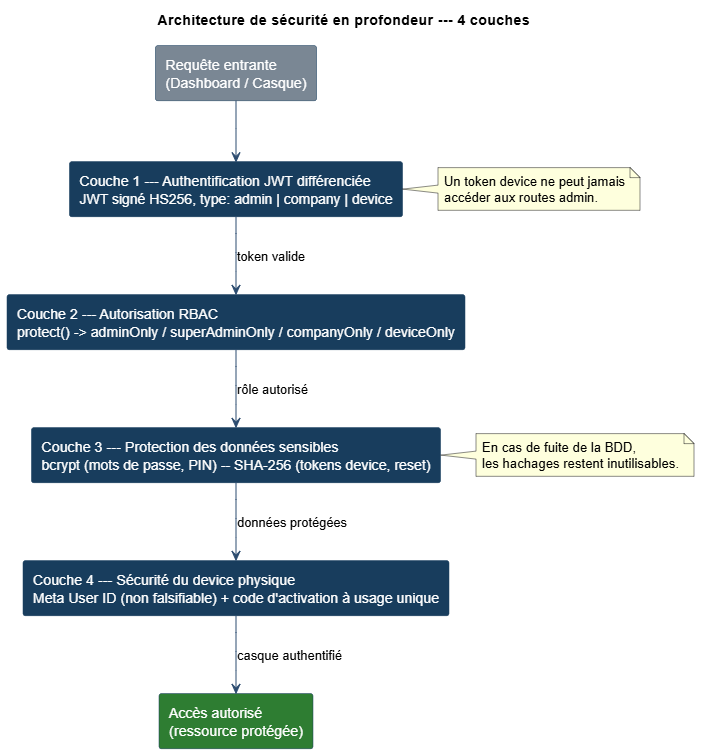
\includegraphics[width=0.85\textwidth]{../images/securite4couches.png}
  \caption{Architecture de sécurité en profondeur à quatre couches}
  \label{fig:securite}
\end{figure}

\subsubsection{Couche 1 --- Authentification JWT différenciée}

Le payload JWT encode le type d'acteur~: \texttt{\{id, type: 'admin'|'company'|'device', role?\}}.
Cette différenciation garantit qu'un token de type \texttt{device} ne peut jamais accéder
aux routes réservées aux admins, même en cas d'interception.

\begin{table}[H]
  \centering
  \begin{tabular}{lll}
    \toprule
    \textbf{Acteur} & \textbf{Type} & \textbf{Durée} \\
    \midrule
    Admin (superadmin / staff) & admin   & 7 jours \\
    Company (dashboard)        & company & 7 jours \\
    Device (casque Meta Quest~3) & device & 1 an \\
    \bottomrule
  \end{tabular}
  \caption{Tokens JWT par acteur}
  \label{tab:jwt_tokens}
\end{table}

Le token device a une durée d'un an car le casque est un device fixe appartenant à
l'entreprise (pas à l'employé individuel). Supprimer le token à chaque changement
d'employé forcerait une réactivation à chaque session, ce qui est opérationnellement
absurde.

\subsubsection{Couche 2 --- Autorisation RBAC}

Les middlewares Express forment une chaîne de contrôle d'accès~:

\begin{itemize}
  \item \texttt{protect()}~: vérifie et décode le JWT.
  \item \texttt{adminOnly()}~: vérifie \texttt{type === 'admin'}.
  \item \texttt{superAdminOnly()}~: vérifie \texttt{role === 'superadmin'}.
  \item \texttt{companyOnly()}~: vérifie \texttt{type === 'company'}.
  \item \texttt{deviceOnly()}~: vérifie \texttt{type === 'device'}.
\end{itemize}

\subsubsection{Couche 3 --- Protection des données sensibles}

\begin{itemize}
  \item \textbf{bcrypt 10 rounds}~: appliqué aux mots de passe Company/Admin et aux
    PINs des employés. 10 rounds $\approx$ 100~ms, délai intentionnel rendant les
    attaques brute force coûteuses en temps.
  \item \textbf{SHA-256 pour les tokens device}~: le token brut (plain) est exposé
    une seule fois, pendant 60 secondes. Seul son hash est stocké en base. En cas
    de compromission de la BDD, les tokens hachés sont inutilisables.
  \item \textbf{SHA-256 pour le reset password}~: même logique, avec expiration de
    30 min.
\end{itemize}

\subsubsection{Couche 4 --- Sécurité du device physique}

\begin{itemize}
  \item \textbf{Meta User ID}~: identifiant matériel unique fourni par le SDK Oculus,
    stable et impossible à falsifier (contrairement à \texttt{deviceUniqueIdentifier}
    qui peut changer après un factory reset).
  \item \textbf{Code d'activation}~: 6 chiffres aléatoires, expire après 15 minutes.
    Saisi manuellement par l'admin dans le dashboard.
\end{itemize}

\subsection{Cas d'utilisation --- Descriptions textuelles}

\begin{ucbox}{Activer un casque Meta Quest~3}
  \begin{tabular}{lp{9cm}}
    \textbf{Pré-conditions} & Casque physiquement présent, admin Staff connecté. \\
    \textbf{Acteur}         & Staff Admin Tynass. \\
    \textbf{Scénario}       &
      1. Unity envoie le Meta User ID à \texttt{POST /request-activation}. \newline
      2. Backend génère un code 6 chiffres aléatoire (expire 15 min). \newline
      3. Admin saisit le code dans la DevicesPage du dashboard. \newline
      4. Backend génère un JWT device (1 an) + stocke le hash SHA-256. \newline
      5. Unity appelle \texttt{POST /check} et reçoit le token brut (60~s). \newline
      6. Token stocké dans PlayerPrefs (permanent). \\
    \textbf{Exceptions}     & Code expiré (15 min) → admin régénère un nouveau code. \\
    \textbf{Post-conditions}& Casque actif en BDD, token persistant sur le casque. \\
  \end{tabular}
\end{ucbox}

\vspace{0.5cm}

\begin{ucbox}{Login employé via casque VR}
  \begin{tabular}{lp{9cm}}
    \textbf{Pré-conditions} & Casque activé, employee créé avec accessCode + PIN. \\
    \textbf{Acteur}         & Employé (via Meta Quest~3). \\
    \textbf{Scénario}       &
      1. Employé saisit son accessCode (format XX-001) via le panel. \newline
      2. Unity valide le format (Regex \texttt{\^{}[A-Z]\{2\}-\textbackslash d\{3\}\$}). \newline
      3. Employé saisit son PIN 4 chiffres via le numpad. \newline
      4. Unity envoie \texttt{POST /api/company/employees/login} avec
         \texttt{device\_token}. \newline
      5. Backend vérifie le PIN (\texttt{bcrypt.compare}) et retourne
         \texttt{employee + auth\_token}. \newline
      6. AppSession stocke les données employé. \\
    \textbf{Exceptions}     & Code invalide → message d'erreur. PIN incorrect → rejet. \\
    \textbf{Post-conditions}& Employé connecté, AppSession initialisée, ModulesPanel
                              chargé. \\
  \end{tabular}
\end{ucbox}

\vspace{0.5cm}

\begin{ucbox}{Soumettre une session de formation}
  \begin{tabular}{lp{9cm}}
    \textbf{Pré-conditions} & Simulation terminée, données collectées dans AppSession. \\
    \textbf{Acteur}         & Système Unity (automatique). \\
    \textbf{Scénario}       &
      1. \texttt{OnboardingManager} calcule le score final. \newline
      2. AppSession contient~: trainingId, employeeId, startedAt, score, criteria[]. \newline
      3. Unity appelle \texttt{POST /api/sessions/submit} (auth\_token dans le header). \newline
      4. Backend calcule \texttt{durationSeconds} (côté serveur, horloge fiable). \newline
      5. Backend incrémente \texttt{attemptNumber} via le pre-save hook. \newline
      6. Session stockée en BDD, visible dans le dashboard admin. \\
    \textbf{Exceptions}     & Perte Wi-Fi → retry automatique via TynassApiClient. \\
    \textbf{Post-conditions}& Session persistante, statistiques mises à jour. \\
  \end{tabular}
\end{ucbox}

\subsection{Diagrammes de séquence}

La figure~\ref{fig:seq_activation} illustre le déroulement complet de l'activation
d'un casque, depuis la demande initiale envoyée par l'application Unity jusqu'à la
récupération du jeton sécurisé.

\begin{figure}[H]
  \centering
  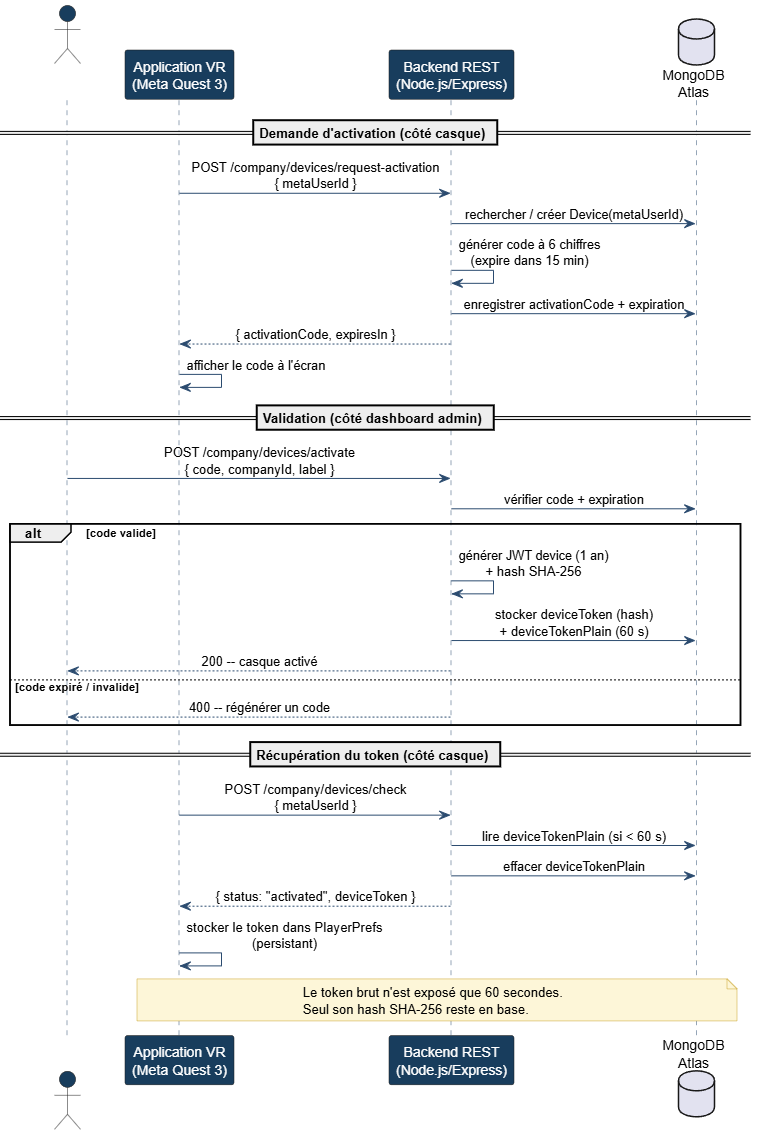
\includegraphics[width=0.9\textwidth]{../images/seqActivation.png}
  \caption{Diagramme de séquence --- activation d'un casque}
  \label{fig:seq_activation}
\end{figure}

\begin{figure}[H]
  \centering
  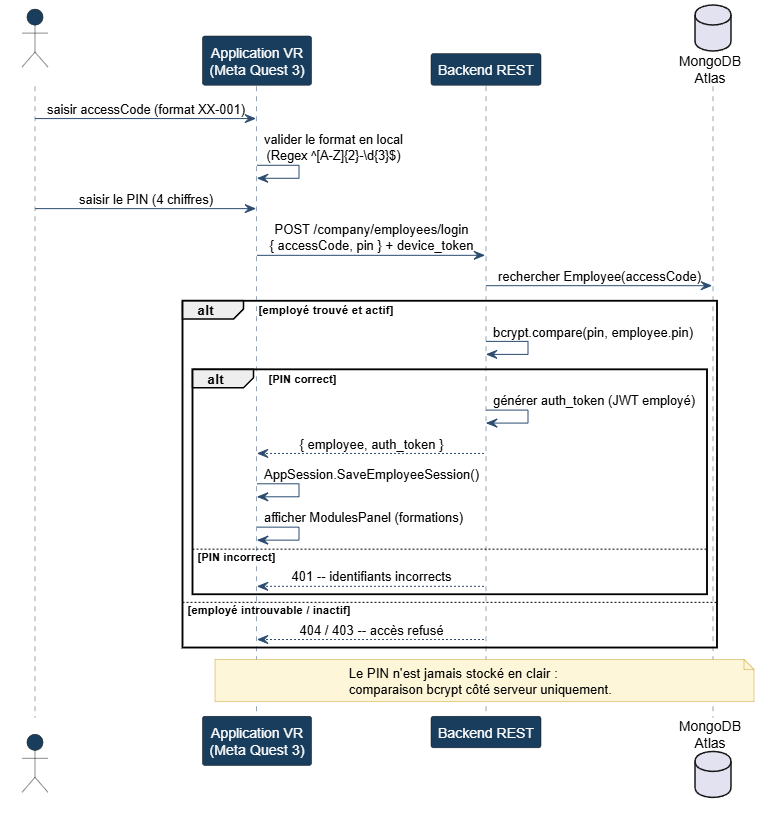
\includegraphics[width=0.9\textwidth]{../images/seqLogin.png}
  \caption{Diagramme de séquence --- login employé}
  \label{fig:seq_login}
\end{figure}

\section{Implémentation de l'itération~1}

Cette section détaille la mise en œuvre du backend~: la structure du projet selon le
patron MVC, les principales routes de l'API REST, et les fonctionnalités clés développées.

\subsection{Structure du projet --- Architecture MVC}

\placeholder{Arborescence des dossiers (à insérer)}

Le projet backend est organisé selon le pattern MVC~:

\begin{itemize}
  \item \texttt{models/}~: 8 schémas Mongoose (Company, Admin, Training, Session,
    Employee, Device, Counter, Quiz).
  \item \texttt{controllers/}~: logique métier séparée par domaine (admin.auth,
    company.auth, admin.companies, admin.trainings, session, employee, device).
  \item \texttt{routes/}~: points d'entrée REST groupés par acteur.
  \item \texttt{middleware/}~: \texttt{auth.middleware.js} avec les 5 guards.
  \item \texttt{utils/}~: \texttt{sendEmail.js} (Nodemailer).
\end{itemize}

\subsection{API REST --- Tableau des endpoints}

Le tableau~\ref{tab:endpoints} présente un extrait des routes principales de l'API.

\begin{table}[H]
  \centering
  \begin{tabularx}{\textwidth}{llXl}
    \toprule
    \textbf{Méthode} & \textbf{Route} & \textbf{Description} & \textbf{Auth} \\
    \midrule
    \multicolumn{4}{l}{\textit{Authentification Admin}} \\
    POST & \texttt{/api/admin/auth/setup} & Créer le 1er superadmin & Public \\
    POST & \texttt{/api/admin/auth/login} & Login admin & Public \\
    GET  & \texttt{/api/admin/auth/me} & Profil admin courant & Admin \\
    \midrule
    \multicolumn{4}{l}{\textit{Gestion Entreprises}} \\
    GET  & \texttt{/api/admin/companies} & Lister toutes les entreprises & Admin \\
    POST & \texttt{/api/admin/companies} & Créer une entreprise & Admin \\
    PATCH& \texttt{/api/admin/companies/:id} & Modifier une entreprise & Admin \\
    POST & \texttt{/api/admin/companies/:id/trainings} & Assigner une formation & Admin \\
    \midrule
    \multicolumn{4}{l}{\textit{Activation Casque}} \\
    POST & \texttt{/api/company/devices/request-activation} & Générer code 6 chiffres & Device \\
    POST & \texttt{/api/company/devices/activate} & Activer avec le code & Admin \\
    POST & \texttt{/api/company/devices/check} & Récupérer device token & Device \\
    \midrule
    \multicolumn{4}{l}{\textit{Login Employé}} \\
    POST & \texttt{/api/company/employees/login} & Login code + PIN & Device \\
    GET  & \texttt{/api/company/devices/trainings} & Formations du casque & Device \\
    \midrule
    \multicolumn{4}{l}{\textit{Sessions}} \\
    POST & \texttt{/api/sessions/submit} & Soumettre une session & Device \\
    GET  & \texttt{/api/sessions/stats} & Statistiques agrégées & Admin/Company \\
    \bottomrule
  \end{tabularx}
  \caption{Endpoints API --- extrait des routes principales}
  \label{tab:endpoints}
\end{table}

\subsection{Fonctionnalité clé --- Système d'activation du casque}

Le système d'activation est la fonctionnalité la plus originale du backend. Il repose
sur l'identifiant hardware Meta User ID, fourni par le SDK Oculus Platform et
impossible à falsifier. Le flow complet est le suivant~:

\begin{enumerate}
  \item L'application Unity envoie le Meta User ID au backend via
    \texttt{POST /request-activation}.
  \item Le backend génère un code aléatoire de 6 chiffres, le stocke haché (SHA-256)
    avec une expiration de 15 minutes, et retourne le code à l'affichage (pour l'admin).
  \item L'admin saisit ce code dans la DevicesPage du dashboard.
  \item Le backend vérifie le code, génère un JWT device (1 an), stocke le hash
    SHA-256 en BDD et expose le token brut pendant 60 secondes maximum.
  \item Unity appelle \texttt{POST /check}, récupère le token brut et le stocke
    dans PlayerPrefs. Le token brut est immédiatement effacé côté serveur.
\end{enumerate}

\subsection{Fonctionnalité clé --- Compteur atomique (accessCode)}

L'accessCode des employés suit le format XX-001 (2 lettres initiales de l'entreprise
+ numéro auto-incrémenté). Pour éviter les race conditions lors de créations
simultanées, le backend utilise la commande MongoDB
\texttt{findOneAndUpdate(\{key\}, \{\$inc: \{seq: 1\}\}, \{upsert: true, new: true\})},
garantissant une incrémentation atomique sans doublons.

\section{Difficultés et solutions}

\begin{table}[H]
  \centering
  \begin{tabularx}{\textwidth}{lXX}
    \toprule
    \textbf{Défi} & \textbf{Problème} & \textbf{Solution} \\
    \midrule
    Race condition & Deux employés créés simultanément pouvaient recevoir le même
                     accessCode (\texttt{countDocuments} non atomique). &
                     Migration vers Counter + \texttt{\$inc} MongoDB~: opération
                     atomique garantissant l'unicité. \\
    \midrule
    Sécurité token device & Stocker le device token en clair en BDD représentait
                            un risque en cas de compromission. &
                            SHA-256 permanent pour le stockage, token brut exposé
                            60~s uniquement puis effacé. \\
    \midrule
    UnityWebRequest 4xx & Unity traitait les réponses HTTP 4xx comme des erreurs
                          réseau sans lire le body JSON. &
                          Restructuration des réponses backend~: toujours
                          retourner un body JSON lisible même sur les erreurs. \\
    \midrule
    Pre-save hook & Utiliser \texttt{async function(next)} dans un hook
                    Mongoose async causait l'erreur
                    \og~next is not a function~\fg. &
                    Suppression du paramètre \texttt{next}~: en Mongoose,
                    les hooks async gèrent automatiquement la promesse. \\
    \bottomrule
  \end{tabularx}
  \caption{Difficultés rencontrées et solutions --- Itération~1}
  \label{tab:dificultes_s1}
\end{table}

\section{Évaluation de l'itération~1}

\begin{table}[H]
  \centering
  \begin{tabularx}{\textwidth}{Xl}
    \toprule
    \textbf{Élément validé} & \textbf{Statut} \\
    \midrule
    Authentification différenciée des trois acteurs (Admin, Company, Device) & Fonctionnel \\
    Activation d'un casque via code à 6 chiffres + jeton haché SHA-256 & Fonctionnel \\
    Login employé (code d'accès + PIN) & Fonctionnel \\
    Enregistrement et restitution des sessions de formation & Fonctionnel \\
    Agrégation des statistiques par formation et par entreprise & Fonctionnel \\
    Tests des endpoints via Postman & Validé \\
    \bottomrule
  \end{tabularx}
  \caption{Validation fonctionnelle --- Itération~1}
  \label{tab:eval_s1}
\end{table}

\placeholder{Capture Postman --- Réponse POST /api/company/devices/check (à insérer)}

\placeholder{Capture MongoDB Compass --- Collections créées (à insérer)}

\section{Conclusion}

Cette première itération a livré le backend complet de \tynassit{}, déployé sur Render
(\texttt{tynassit-backend-pfe.onrender.com}). L'architecture de sécurité à 4 couches
garantit l'isolation des acteurs et la protection des données sensibles. Le système
d'activation des casques, combinant identifiant matériel Meta User ID et code
d'activation à usage unique, constitue la fonctionnalité la plus originale du projet.
